\chapter[数字要能作证：硬件层开发与硬件度量]{数字要能作证：\\硬件层开发与硬件度量}

\begin{noteblock}
Semantica 绑定： 本章保存硬件度量的概念、算例与证据纪律；唯一机器语义是
\nolinkurl{semantica.chapter_packages.vol2.ch06}，主场景为
\nolinkurl{semantica.vol2.ch06.scenario.primary}。本体、CQ、查询、Shape、正反案例、规则、
oracle、manifest、PROV 与 receipt 只在 Semantica。当前为 \nolinkurl{partial}、release
\nolinkurl{blocked}；算例 oracle 通过不构成 FMEDA 充分性、真实硬件指标或放行结论。
\end{noteblock}

\begin{center}
\vspace{0.2em}
\chapterartfade{%
\adjustbox{max size={0.88\linewidth}{0.27\textheight}}{
\includegraphics{figures-imagegen/art-ch06-v01.png}}%
}
\vspace{0.35em}
\end{center}

\begin{noteblock}
\textbf{【导读】}
第 5 章散场时，系统层把需求和预算分了下去：软件领走一叠要实现的承诺，
硬件领到的却是一串数字——两个百分数、一个概率上限，外加“必须达标”四个字。
本章陪硬件团队把这串数字走一个来回：先弄清数字背后的需求从哪里来；
再看“失效率”这个数是谁的、按什么条件成立；然后立起一笔五个去向的账，
亲手把两个度量算出来，再算一次“加一个监控器能好多少”；
最后在一场审核留下的旧伤疤前停下来，看清一个没有来源的数字能造成什么。
读完本章，你应当能对任何一个写在报告里的数字问出五个问题——
对象是谁、方法是什么、单位是什么、不确定度多大、来源在哪——
并判断它此刻是站在证据的位置上，还是只是恰好站在那个位置上。
\end{noteblock}

\Needspace{6\baselineskip}
\section{预算到手的那个下午}

小唐抱着一摞文件走进硬件组，是个周二下午。系统层的分配工作收了尾，
分给硬件的那一份摆上了吴工的桌面：一叠分配给硬件的技术安全需求，
以及一页度量预算——针对“不产生非预期助力”这条最高等级的安全目标，
单点故障度量 SPFM 不低于百分之九十九，潜伏故障度量 LFM 不低于百分之九十，
随机硬件失效导致安全目标违背的平均概率 PMHF 不超过每运行小时亿分之一的量级。

小唐把预算页抽出来，半开玩笑半认真地说：“说实话，我挺羡慕你们硬件的。
系统层为‘需求接没接住’吵了三个月，全是判断题；你们这儿多干净——
三个门限写得清清楚楚，算出来，过线，签字。数字不会骗人。”

这句话一点都不外行。把验收从“我觉得可以”变成客观的数值比较，
本来就是几代工程管理努力的方向；数字确实比形容词可审得多，
一个百分数至少可以被复算，而“充分”“足够”连复算的入口都没有。
如果这个行业把随机失效的管理压缩成三个门限，那一定是因为门限背后
有一整套撑得起它的方法——问题只在于，拿到门限的人还记不记得那套方法。

硬件负责人吴工没有接话。他干了二十多年硬件，从画电源板起家，
上一代转向平台的控制器就是在他手里从原理图走到量产的。
他有个全组皆知的怪癖：任何表格必须有一列“出处”，
没有出处的数字不许过夜。新人听过这个怪癖的好几种来历版本，
真实的那个版本，本章后面会讲到。

那天下午，吴工只是把预算页翻过来，在背面竖着写了五个词：
对象？方法？单位？不确定度？出处？然后对小唐说：“数字不会骗人，
但数字也不会自己作证。要让 99\% 这个门限有意义，
得先知道硬件被要求做到什么——不是‘达标’，是需求。需求从哪里来？”

\Needspace{6\baselineskip}
\section{机制要有上游：硬件安全需求怎么写}

硬件层的开发不是“做一块达标的板子”。它同时欠着三笔账：
把技术安全概念里分给硬件的承诺实现出来；分析随机硬件故障和它们的影响；
和软件把接口协调清楚。三笔账在转向系统上正好拧在一起——
转矩通路上的诊断状态由硬件产生，软件要正确读到并作出反应，
单独优化任何一端，都证明不了整条安全路径成立。

第一笔账落到纸上，就是硬件安全需求：从分配给硬件的技术安全需求往下派生，
把硬件要守的承诺写成可验证的句子。它们大致管五类事：控制硬件内部的失效
（时钟异常时，看门狗要在规定时间内动作）；控制或容忍来自外部的失效
（传感器输入开路时，输入级要进入可诊断的状态）；满足其他元素托付过来的需求
（驱动级要向软件提供可用的故障状态）；把内外部失效检出并通报出去，
而不是悄悄遮蔽；以及不属于机制的约束——随机失效的目标值、禁止的行为、
连接器和线束上的设计措施。

写需求看起来是文书工作，跳过它的诱惑很实在。一种想法是靠经验：
“资深工程师看一眼架构，该加的监控自然会加。”这话对了一半——
经验确实是机制的重要来源，但经验没法被审：新人看不出哪个监控是必须的，
供应商猜不到你默认了哪些保护，下个月来的审核员更没法核对
“工程师觉得应该有”。另一种想法是抄成熟平台：“上一代的机制清单搬过来，
错不了。”也对了一半——成熟平台的机制清单是真金白银换来的，
但它回答的是上一个产品的问题；架构换了、需求换了、
分配换了，抄来的机制可能守着一扇已经不存在的门，
而新开的门没人守。两条路的共同缺陷是一样的：机制和需求之间断了线，
出了事没人说得清“这个监控是为哪条承诺存在的”，
没出事也没人说得清“哪条承诺还没有机制”。

\textbf{安全机制不是设计师的善意，而是需求的债务：失效分析表里每一行“机制”，都必须能指出一条要求它存在的需求；反过来，每一条分给硬件的承诺，都必须能指出谁在替它站岗。}

这条纪律还有两处容易记错的边界。其一，机制不必是纯硬件——
硬件出诊断信号、软件做反应，是最常见的组合；正因为如此，
硬件和软件负责人要共同核定接口清单：硬件给出的诊断位，
软件真的会去读吗？读到之后来得及反应吗？一个覆盖率写着 90\% 的机制，
如果软件根本没订阅它的状态位，覆盖率就只是表格里的装饰。
其二，需求追溯不必挂到每颗电阻——承诺追到最低层的硬件组件就够了；
但失效分析可以继续往下挖到单个元器件和它的失效模式。
这是两笔不同的账：追溯回答“谁实现这条承诺”，
分析回答“物理世界怎样破坏这条承诺”。把分析粒度误当追溯义务，
会造出几千行没人维护的假精确矩阵；把追溯下界误当分析下界，
又会漏掉真正危险的那颗小器件。

需求有了，机制有了户口，表格的下一列轮到失效率——
每个器件、每条路径，一年到头到底坏得多勤？这个数从哪里来？
最顺手的答案是：查手册。

\Needspace{6\baselineskip}
\section{手册上的失效率，是谁的失效率}

小蔡最近被派到硬件组轮岗。填失效分析表填到电阻那几行时，
她觉得这是全表最轻松的部分：“这个好办，手册上查得到。
手册说这类电阻零点几个 FIT，那 R17 就是零点几个 FIT，填进去就行了。”

先说单位。FIT 是失效率的行业单位：1 FIT 表示每十亿器件小时一次失效——
它是速率，不是“十亿小时后必坏”的寿命承诺。小蔡的话也一点不外行：
工业界公认的手册数据本来就是失效率的正规来源之一，
查手册正是正确动作的第一步。她只是不知道，她随手举的这个例子，
恰好是全公司最有名的一颗电阻。

R17——就是几个月前那场乌龙的主角，一个和候选代号只差一个字母的位号，
让七个人开了四十分钟紧急会。那次虚惊的正文只有一句话：
这颗电阻的某个来料批次，失效率略超门限，按正常流程处置。
现在把这句话放到手册数字旁边，问题自己站了出来：
手册说这类电阻零点几个 FIT，那个批次却实实在在越了线——
手册错了吗？没有。手册的数字是一个关于“这类器件、在声明的条件下、
按声明的统计口径”的总体陈述，它从来没有听说过你的这个批次、
你的这块板、你的发动机舱。

那怎么办？会议室里的自然对策照例有几条，值得逐一试过。

第一条：换一本更保守的手册，取更大的数，“保守总不会错”。
错。首先，保守的代价是真实的——失效率抄大一倍，预算立刻吃紧，
逼着你在别处加机制、加成本，而这些机制自己也会带来新的失效率；
其次，对于按比例计算的度量，把所有数一律放大并不自动保守：
分子分母一起变大，比值未必往安全的方向走。保守是一种需要逐项论证的判断，
不是一种可以批发的美德。

第二条：不用手册，用现场统计，“真实数据总比手册强”。
方向是对的，门槛常被略过：现场统计要成为证据，得先证明可比——
统计对象和你的器件是不是同一类、同一工艺？运行条件相当吗？
样本量撑得起结论吗？一个新设计根本还没有现场，
上一代产品的现场数据用过来，中间隔着的每一处差异都要说明。

第三条：让老师傅拍一个，“他看了三十年器件”。经验可以进账，
但要先立判据后出数：估计的依据是什么、和哪些已知数据对过、
不确定的范围多大。先有数再找理由的专家判断，不是判断，是背书。

三条路都通向同一个要求：一个失效率要能用，光有数值不够，
它得随身带着自己的身份——对象（哪类器件、哪个工艺、哪个批次口径）、
条件（什么温度、什么应力、什么任务剖面）、时间基准（按运行小时
还是日历小时——一辆车一年运行几百小时，日历却走八千七百多小时，
两种口径差着一个数量级，不换算就相加是把米和英尺加在一起）、
方法（手册、现场统计还是专家判断）、以及不确定度（这个数附近有多宽的雾）。
还有一条最容易忘的：数字的前提在设计这边也要守住——
手册数字假定器件在额定范围内工作，如果你的设计让那颗电容长年超温，
手册抄得一字不错，前提已经死了。

\textbf{失效率不是器件的属性，是一句主张：“某类对象，在声明的条件与时间基准下，按某种方法统计，失效速率是多少、不确定多少。”把数抄走、把这句话留下，数据就退化成了装饰。}

小蔡在表格里给 R17 填上了数，也照吴工的规矩在“出处”一栏
写上了手册版本和适用条件。然后她发现了下一件怪事：
表里那段没有监控的供电路径，失效率只有 2 FIT，全表最小，
却被吴工标成了最扎眼的红色；旁边失效率大它几十倍的行，反而安然无事。
同样是 FIT，为什么去向差这么多？

\Needspace{6\baselineskip}
\section{同样 2 FIT，去向为什么不同}

因为度量在乎的不是数字的大小，而是失效的去向。
对着一个确定的安全目标，每一份失效率都要被问三个问题，
然后判进五个去向之一。

第一问：它单独发生，会不会直接把安全目标顶穿？
那段无监控供电路径的答案是会——它一旦失效，
控制器可能在没有有效控制的情况下输出非预期助力，
而且没有任何机制拦它。这样的份额叫\textbf{单点故障}贡献：
数值再小，性质最重。如果一个元素有机制罩着、
但机制罩不住的那部分仍能单独顶穿目标，漏网的份额叫\textbf{残余故障}。

第二问：它需要和另一个独立故障凑在一起才能顶穿吗？
凑对才危险的，进多点故障的账——再按第三问分成两半：
在规定窗口内能被检出（或被驾驶员察觉）的，叫\textbf{可检出的多点故障}；
在窗口内始终无声无息的，叫\textbf{潜伏的多点故障}。
潜伏是危险的蓄水池：第一重故障躺在暗处，
系统看起来一切正常，直到第二重故障到来。

第三问都不沾的——发生了也不显著增加目标被违背的概率——才叫\textbf{安全故障}。

小蔡立刻想到了那个最顺手的修法：“给供电路径加个监控不就行了？
被监控了，就是安全故障了。”这个直觉几乎人人有过，
它跳过了至少四个问题：监控器盖得住这条路径的哪些失效模式，
盖不住的剩几成？检出之后，谁去控制后果——来得及吗？
“来得及”用什么衡量？监控器自己坏了怎么办？
四个问题没答之前，“有监控”什么也不改变。

另一个顺手的错法是拿覆盖率当判决：“这机制覆盖率 90\%，
所以 90\% 都安全了。”覆盖率只回答“机制对这组失效模式盖住了多少”，
盖住的那部分去哪个账——是安全、是可检出多点、还是别处——
要看后果是否受控、组合关系是否成立、时间是否来得及，
覆盖率一个数决定不了。

时间是这里最硬的裁判，而且是两只不同的钟。第一只钟属于整车：
从故障发生到危险可能出现，中间有多长的窗口留给检测加反应？
这个窗口由车辆动力学和危害情境决定，机制再快也改变不了它——
顺带说明，转向这一项的窗口值此刻还压在系统层的待定清单上，
所以本章所有与它挂钩的覆盖信用都注明“以窗口定值为准”。
第二只钟管潜伏：第一重故障允许在暗处躺多久，
才不至于和第二重故障凑成不可接受的风险？自检一天跑一次还是一个点火周期跑一次，
决定一大笔失效率是记在“可检出”还是记在“潜伏”。
一个监控器可以“最终总会报警”，却在两只钟上都拿不到信用：
报警慢过第一只钟，直接后果的信用没有；自检慢过第二只钟，
“可检出多点”的信用也没有。

\textbf{分类不是器件的户籍，是一次裁决：同一个失效，换一个安全目标、换一套机制、换一只钟，判决就要重写；而每一份进了账的失效率都必须有去向，一分不许丢，一分不许重。}

供电路径的 2 FIT 之所以刺眼，正因为它此刻判在单点故障——
全表几百个 FIT 里，真正顶在咽喉上的就是这 2 FIT。
账立到这里，两个百分数终于可以出场了：它们就是从这笔五个去向的账里，
用两次除法算出来的。算一遍，比读十遍定义都清楚。

\Needspace{6\baselineskip}
\section{把账算一遍：400 FIT 的底账}

吴工把组里的人聚到白板前，用一份刻意缩小的教学底账做走查——
真实项目的失效分析有几百行，这里聚合成四个元素，
数字都是合成的，方法是真的。账面如下（单位：FIT）：

\begin{center}
\begingroup\small
\setlength{\tabcolsep}{4pt}
\begin{tabularx}{\linewidth}{@{}XXXXXXX@{}}
\toprule
元素 & 总失效率 & 单点 & 残余 & 可检出多点 & 潜伏多点 & 安全 \\
\midrule
传感器 & 100 & 0 & 5 & 20 & 5 & 70 \\
控制器 & 200 & 0 & 8 & 60 & 12 & 120 \\
驱动功率级 & 98 & 0 & 5 & 20 & 3 & 70 \\
无监控供电路径 & 2 & 2 & 0 & 0 & 0 & 0 \\
\textbf{合计} & \textbf{400} & \textbf{2} & \textbf{18} & \textbf{100} & \textbf{20} & \textbf{260} \\
\bottomrule
\end{tabularx}
\endgroup
\end{center}

每一行五个去向加起来等于总失效率，合计行也闭合。
先说清这个闭合能证明什么：它只证明没有把失效率算丢或算重，
不证明每个数判得对——就像财务报表的借贷平衡，假账也能平，
但不平的账一定不能签。

单点故障度量 SPFM 问的是：全部纳入的失效率里，
\Needspace{8\baselineskip}
有多少\textbf{没有}以单点或残余的方式直接威胁这个安全目标？

\nopagebreak[4]
\begin{codebox}
\begin{Verbatim}[fontsize=\small,breaklines=true,breakanywhere=true,breaksymbolleft={},breaksymbolright={}]
SPFM = 1 − (2 + 18) / 400 = 95.00%
\end{Verbatim}
\end{codebox}

吴工让小蔡接着算潜伏故障度量 LFM。她照着直觉写下 1 - 20/400，
得了 95\%。吴工摇头：“分母错了。”LFM 问的是另一件事：
把已经被 SPFM 盯住的单点和残余扣掉之后，
在剩下的空间里，还有多大比例的失效在潜伏？
\Needspace{8\baselineskip}
分母要先减去那 20 FIT 的单点与残余：

\nopagebreak[4]
\begin{codebox}
\begin{Verbatim}[fontsize=\small,breaklines=true,breakanywhere=true,breaksymbolleft={},breaksymbolright={}]
LFM = 1 − 20 / (400 − 2 − 18) = 1 − 20/380 = 94.74%
\end{Verbatim}
\end{codebox}

差得不多，性质全变：用错分母，等于让同一笔危险贡献在两个度量里
各被稀释一次，问题就悄悄换掉了。分母还有一个更隐蔽的软肋——
想让 SPFM 变好看，最省力的路不是消灭危险失效，
而是往分母里灌无关的硬件：多算进一堆与安全目标毫无瓜葛的器件，
总失效率涨了，比值自然“改善”。这就是为什么评审第一件事是核范围：
分母里装的必须是“可能显著促成或阻止这个安全目标被违背”的硬件，
一件不多，一件不少。

\textbf{度量是除法，而除法的全部诚实都在分母里：分母的定义换一个字，度量回答的问题就换了一个；分母的范围松一寸，绿色就便宜一寸。}

对照预算：SPFM 95.00\%，门限 99\%，没过；LFM 94.74\%，门限 90\%，过了。
账面清楚地指出病灶——分子里那 2 FIT 的单点贡献和 18 FIT 的残余贡献。
没过线怎么办？自然的动作是给那段裸奔的供电路径加机制。
下一节就加：加一个监控器，账到底能变好多少？


\begin{noteblock}
\textbf{读图任务}：沿左侧总流量跟随四条宽度不同的支流，确认安全侧、已监控、残余与潜伏都是同一总体的去向。
\end{noteblock}

\begin{center}
\begin{minipage}{\linewidth}
\centering
\adjustbox{max size={\linewidth}{0.78\textheight}}{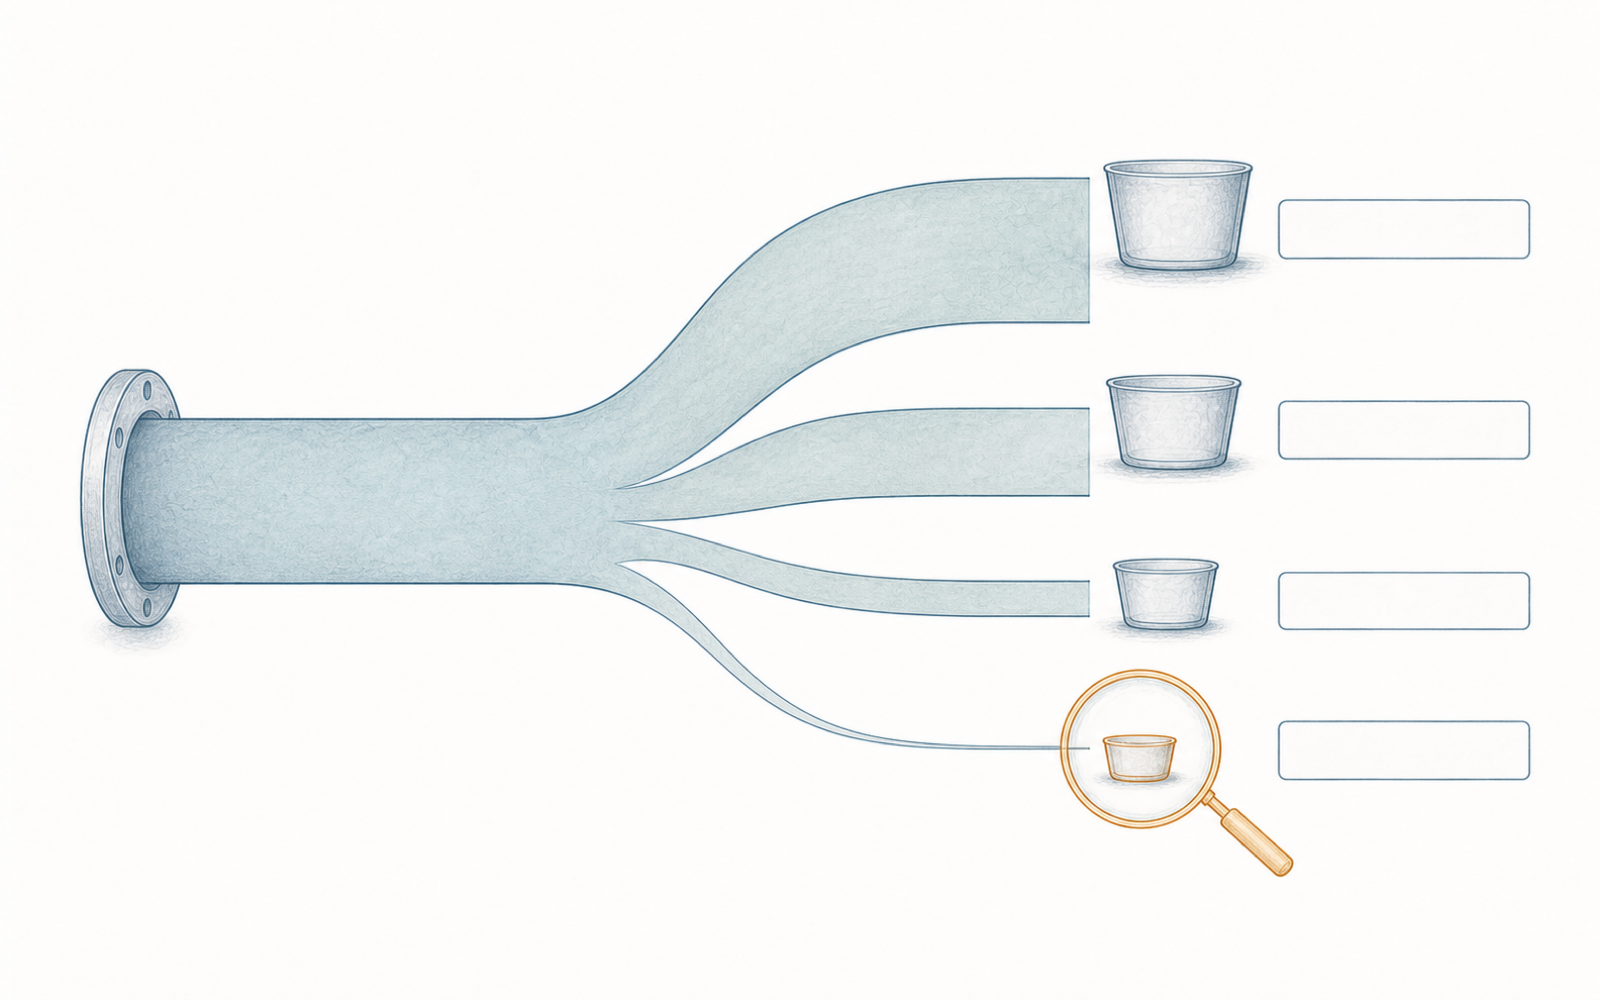
\includegraphics{figures-imagegen/ch06-fig01-failure-rate-flow-v01.png}}
\captionof{figure}{评价硬件度量时，关键不是只报一个总数，而是说清分类规则与每一单位的去向。小分支也可以决定分子、分母和最终结论。}
\end{minipage}
\end{center}


\begin{noteblock}
\textbf{图后判断}：这是教学性流量账，不是真实元件失效率报告。它不给出 SPFM、LFM 或 PMHF 数值，也不证明诊断假设已被验证。
\end{noteblock}

\Needspace{6\baselineskip}
\section{加一个 U7，只好了零点四八}

设计变更是：新增一颗供电监控比较器，位号 U7，
自身失效率取合成值 3 FIT。走查开始前，吴工先钉死一个边界：
\textbf{原来的 400 FIT 里没有 U7}——加装之后总失效率是 403，不是 400。
这句啰嗦话关掉了一个危险的歧义：如果 U7 原本就藏在某行里、
现在又额外加 3 FIT，同一颗器件就在分母里被算了两次。

第一步，原供电路径的 2 FIT 迁账。假设 U7 对相关危险模式的覆盖率是 90\%，
且检出与反应赶得上两只钟、U7 与被监控路径确实独立——注意，
这些全是要逐条拿证据的假设，不是“装了监控器”自动附赠的性质。
在假设成立的前提下：1.8 FIT 迁去“可检出多点”，0.2 FIT 留作残余。
小蔡问：“为什么不能直接 2 \(\times\) 90\% 搬走完事？”因为覆盖率不授权迁账：
被盖住的 1.8 FIT 要逐模式核实后果受控、组合关系成立、时间来得及，
才有资格坐进多点的账；三个前提缺一个，就退回原地。

第二步，U7 自己也要进账——这是最常被赖掉的一笔。
监控器不是天使，它也是硅和焊点。它的 3 FIT 按后果分析拆开：
45\% 的模式不显著增加目标被违背的概率，记安全故障 1.35 FIT；
其余 55\%（1.65 FIT）会让监控功能失灵——这正是典型的多点候选：
U7 悄悄坏了，供电路径再坏，两重凑齐。这 1.65 FIT 里有多少潜伏，
取决于\textbf{谁来监控监控器}：假设由控制器既有的诊断路径检测 U7 的恒高、
漂移等危险模式，且检测周期赶得上第二只钟，则 90\% 即 1.485 FIT
记作可检出多点，剩下 0.165 FIT 是没人照看的部分，老老实实记潜伏。
（这条诊断路径的硬件已在控制器那 200 FIT 里，不再新增分母——
若真实设计要为此加新硬件，新硬件的失效率就得进总账重算。）

\Needspace{8\baselineskip}
第三步，重算。其他元素的 18 FIT 残余没人动过，原样在账上：

\nopagebreak[4]
\begin{codebox}
\begin{Verbatim}[fontsize=\small,breaklines=true,breakanywhere=true,breaksymbolleft={},breaksymbolright={}]
SPFM = 1 − (18 + 0.2) / 403 = 1 − 18.2/403 = 95.48%
LFM  = 1 − (20 + 0.165) / (403 − 18.2) = 1 − 20.165/384.8 = 94.76%
\end{Verbatim}
\end{codebox}

白板前有几秒失望的沉默。加了一颗监控器，SPFM 从 95.00\% 到 95.48\%——
离 99\% 还远。但这半个百分点是诚实的：U7 把最危险的 2 FIT 大部分迁出了分子，
同时带进了自己的 3 FIT，而基线里还有 18 FIT 的残余贡献根本不归它管。
想让数字戏剧性变好，办法有的是——把 U7 的失效率漏掉不记，
把 18 FIT 的残余含糊过去，或者给分母灌水——每一种都能让屏幕变绿，
没有一种能让车变安全。

这笔账真正的价值在于它可以被“单因拷问”：一次只推翻一个假设，
看哪笔信用被撤回。若控制器诊断路径检测 U7 的周期慢过第二只钟，
U7 危险侧的 1.65 FIT 全部转潜伏，LFM 落到约 94.37\%，SPFM 暂时不动；
若检出加反应超过第一只钟的窗口，原路径那 1.8 FIT 的覆盖信用整笔吊销，
必须回去逐模式重判——这里没有一个方便的新百分数可报，
诚实的“待重算”胜过伪精确；若相关失效分析发现 U7 和被监控路径
共享一个能同时放倒两者的原因——同一路供电、同一个基准源——
“两个独立故障”的前提塌了，所有押在它上面的分类和结果一并撤回。

\textbf{机制改变的是分类，不是物理：它自己的失效率必须入账，它挣来的每一分信用都押着一条列得出、也撤得回的假设。}

走查散场前，小唐探头进来问进度，听到 95.48\%，愣了愣：“那就是说，
再迭代几轮设计，把两个百分数都推过线，硬件这块就可以签了？”
吴工这次没有立刻回答。他把马克笔放下，说了一句组里老人都听过的话：
“过线之后，还有一道我欠过债的坎。”

\Needspace{6\baselineskip}
\section{过线之后：那个复制来的数}

先把道理摆出来，再讲那笔债。

SPFM 和 LFM 是比例，而比例天生有一个盲区：它看结构，不看绝对量。
想象两个设计都做到了 99.5\% 的 SPFM——A 的总失效率很低，
B 的总失效率高出一个数量级；同样是 0.5\% 的危险份额，
落到整车上的绝对风险差着十倍。所以标准在比例之外还要一把绝对的尺子：
估计在整个运行寿命内，随机硬件失效平均每运行小时把安全目标顶穿的概率——
行业里叫 PMHF——并给它设概率上限；不走这条路的项目，
也得走另一条：把能顶穿目标的失效原因一个一个拉出来过堂，逐个证明可接受。
两把尺子问的问题不同，谁也替不了谁。而无论哪条路，
都要吃进一大堆输入：架构、每个器件的分类失效率、机制的覆盖、
潜伏的暴露时长。也就是说，\textbf{那个最终写在报告里的概率，是全章这笔账一路诚实算下来的孙子辈}；账断在哪一环，它就悬空在哪一环。

现在讲那笔债。上一代转向平台做客户审核，是好几年前的事。
硬件评估报告里有一个 PMHF 值，写得很漂亮，小于目标上限，绿色。
审核员只问了一句：“这个数是怎么算出来的？”会议室里没有人能答。
翻记录，那个数来自一张电子表格；追表格，那一格是从更早一个项目的
报告里复制来的；再追那份更早的报告，算它的人已经离职，
计算过程没有归档，连当年用的失效率库是哪个版本都无从查起。
一个数字被复制了两代项目，它的出处比它先死了。

会议室里不是没有人替它辩护，而且两句辩护听起来都有道理。
一句是：“两代平台架构差不多，数字的量级不会错。”——
“差不多”恰恰是一个需要论证的判断：差在哪里、差多少、对结果敏感不敏感，
得有一张差异清单撑着；而当年连这张清单都没有，
“差不多”只是一种愿望的语法。另一句是：“这个数当年通过了评审。”——
当年的签字属于当年那个项目、那份报告、那句主张；
签字不能跨项目迁移，就像台架的绿灯不能替别的配置作证。
两句辩护相继失效之后，房间里只剩下那个数字本身：
数值没错——后来重算出来量级确实相当——但在被追问的那一刻，
它拿不出对象、拿不出方法、拿不出单位口径、拿不出不确定度、拿不出来源。
它不是证据，它只是长得像。

代价是实打实的：审核开出正式发现项，评估中断；
随机失效评估从输入开始重建，硬件组补了整整一个季度的证据链；
量产节点顺延，客户那边的信任又花了更久才补回来。
而当年在表格里按下“粘贴”的那个年轻工程师，
是吴工自己。他的上级当时说“先把格子填上，量级差不多，回头补算”，
后来上级离职了，“回头”再也没有来。审核那天，
是吴工站起来说的实话：“这个数是抄来的，我抄的。”
从那以后，他的表格里多了那一列“出处”，
没有出处的数字，在他手下不许过夜。

\textbf{脱离对象、方法、单位、不确定度和来源的数字不是证据——它只是一个恰好站在证据位置上的数；而它站得越久，把它请下来的代价越大。}

顺手多问一层：为什么“先把格子填上”这句话，总是由上级说出口，
而且换一家公司还是有人说？因为在组织的眼睛里，进度看得见，出处看不见。
格子填上的那一刻，汇报立刻多一格绿，好处当场兑现；“这个数从哪来”
要等到几年后有人追问才会显形，而到那时，说“先填上”的人多半已经不在场。
一边是当天结清的奖励，一边是记在别人名下的远期债——账期这样错开，
个人的诚实就得逆着激励游泳。吴工那列“出处”，做的正是把看不见的那一半，
强行搬回看得见的表格里。

这也是给小唐那句“过线就能签”的完整回答。度量过线，
证明的是架构对随机失效的相对覆盖，在声明的范围、账目和假设内成立——
这已经很多，但硬件安全不止这些。比例过了还有绝对概率要问；
随机的账算平了，系统性的故障一分都没碰——画错的原理图、
超额定使用的器件、没定义清楚的接口，这些不是概率现象，
分母再大也稀释不了它们，管它们的是设计规程、评审和验证；
最后，算出结果的人不能自己宣布结果成立，度量和评估的结论
还要过独立的验证评审——公式是分析者按的回车，结论需要另一双眼睛。
签字那一栏真正对应的主张是：“在此对象、此范围、此账目、此假设下，
这些数字说了它们有资格说的话。”——每一个数字都能作证，
但要按它的射程作证。这正是第 1 章那句老话在硬件层的样子。

道理讲完，账也算平，本章按说可以收尾了。
可吴工那列“出处”还悬着一个没人爱问的问题：
这列格子，靠什么保证一直被填、一直填对？

\Needspace{6\baselineskip}
\section{纸面追不上数字的脚}

诚实地看一眼数字在真实项目里的日常旅行：失效率从手册进了分析表，
从分析表聚合进度量计算，度量结果进了评估报告，报告里的结论
被摘进评审胶片，胶片上的绿格子被抄进月度汇报。五段旅程，
每一段都是一次复制，而纸面世界的复制只搬数值，不搬护照——
对象、方法、单位、不确定度、来源，每复制一次就有机会掉一样。
到了汇报那一页，“95.48\%”孤零零站在那里，
它曾经拖着的那一整套前提——400 还是 403 的分母、
两只钟的假设、独立性的前提、“以窗口定值为准”的批注——一样都不剩。
吴工的债，就是这样欠下的：没有人作恶，只是复制了太多次。

纸面世界对此不是没有办法，它的办法就是吴工那样的人：
立规矩（表格必须带出处列）、传习惯（新人第一课先学问来历）、
设关卡（评审时逐个数字问一遍五个问题）。这些办法是真办法——
本章前七节就是它们的展开，这个行业靠它们把随机失效管了几十年，
管得相当好。但它们有一个共同的形状：\textbf{纪律长在人身上，不长在数字身上。}
吴工在的时候，没有出处的数字过不了夜；吴工休假的那两周呢？
换一家供应商呢？表格换一种模板呢？电子表格的单元格从不拒绝粘贴，
文档不会在数字丢掉前提的那一秒弹出警告，
而评审能抓住多少，取决于评审的人恰好想起问哪一格。
一句话：纸面可以\textbf{要求}每个数字带上护照，
却没有力气在数字被复制的那一秒钟\textbf{强制执行}。

这个极限不是硬件独有的。换个世界看一眼就知道：那台环境监测单元
ENV-01 的标定证书上写着“\(\pm\)0.5\%”，这个数被抄进产品手册、
抄进投标文件、抄进客户的验收清单——每一站都该有人问：
对哪个量程、什么温度、距上次标定多久、不确定度怎么给的？
问法和硬件度量的五问一模一样；答案则要在它自己的世界里重新挣。
可迁移的是问法，扛不动的也一样——纸面同样追不上那个数字的脚。

所以本章末尾冻结的，不是答案，是三个交给后半本书的问题：
怎样让一个数字无论被复制到哪里，都被迫带着它的对象、方法、单位、
不确定度和来源，少一样就寸步难行；怎样让“过线”这样的比较结论
自动拴着自己的范围与假设，前提一变，结论自动失效而不是继续变绿；
怎样让每一次复制都留下痕迹，让任何一个数都能反查血缘，
一路追到第一次测量或第一次假设为止。第 16 章会回到这三个问题，
用另一种载体让数字自己扛住这些义务——那是 AI 之后的世界的做法。

而眼前，走廊另一头的问题已经等在那里。小林的软件组也在准备自己的证据，
但他们的桌上没有 FIT，没有失效率手册，没有任何可以聚合的概率——
软件的错误不是随机的，是设计进去的：同一个缺陷，一百万次运行就复现一百万次，
没有“每十亿小时坏一次”可言。硬件的“达标”好歹有两把尺子可算，
软件连尺子都没有——那软件的“通过”，靠什么成立？
第 7 章从这里开始。

导读的承诺可以兑现了。合上书之前，做三件事：
在你手头的任何一份分析或预计表里任选一个失效率，
试着一次写全它的对象、条件、时间基准、方法和不确定度，
看卡在哪一样；找一个正在你的组织里流通的“达标”百分数，
问清它的分母里装了什么、谁批准的范围；再挑一个你确定被复制过的数字，
沿着它的旅程往回走，数一数它每过一站丢了什么。
如果第三件事让你走进了死胡同——记住那个位置，第 16 章会回到那里。


\begin{noteblock}
\textbf{本章注记}：本章的人物、会议、审核事件与全部数字（度量值、失效率、
覆盖率、门限、位号、时间跨度等）均为合成教学材料，不对应任何真实企业、
真实产品或真实个人；400 FIT 底账与 U7 变更算例是刻意缩小的教学账，
不是任何实际产品的分析结果。正文对标准中硬件度量与随机失效评估要求的
转述为自然语言概括，精确定义与适用条件以标准原文为准；
本章不构成对任何实际系统的达标判定或放行结论。
\end{noteblock}
